\documentclass{article}

\usepackage{arxiv}

\usepackage[utf8]{inputenc} % allow utf-8 input
\usepackage[T1]{fontenc}    % use 8-bit T1 fonts
\usepackage{hyperref}       % hyperlinks
\usepackage{url}            % simple URL typesetting
\usepackage{booktabs}       % professional-quality tables
\usepackage{amsfonts}       % blackboard math symbols
\usepackage{amsmath}
\usepackage{microtype}      % microtypography
\usepackage{graphicx}

\title{AI-assisted pharmaceutical analysis of prescriptions combining retrieval-augmented generation and a knowledge-based system}

\author{
	Isen Naiken \\
	CHU Dijon Bourgogne \\
	Dijon, France \\
	\texttt{isen.naiken@chu-dijon.fr} \\
	\And
	Bastian Fouquier \\
	CHU Dijon Bourgogne \\
	Dijon, France \\
	\texttt{bastian.fouquier@chu-dijon.fr} \\
	\AND
	Mathieu Boulin \\
	CHU Dijon Bourgogne \\
	Dijon, France \\
	\texttt{mathieu.boulin@chu-dijon.fr} \\
	\And
	Marie-Pierre Guenfoudi \\
	CHU Dijon Bourgogne \\
	Dijon, France \\
	\texttt{marie-pierre.guenfoudi@chu-dijon.fr} \\
}

\renewcommand{\shorttitle}{AI-assisted pharmaceutical analysis of prescriptions}

\hypersetup{
pdftitle={AI-assisted pharmaceutical analysis of prescriptions combining retrieval-augmented generation and a knowledge-based system},
pdfsubject={cs.CL, cs.AI},
pdfauthor={Isen Naiken, Bastian Fouquier, Mathieu Boulin, Marie-Pierre Guenfoudi},
pdfkeywords={Clinical pharmacy, Medication review, Large language model, Retrieval-augmented generation, Knowledge-based system},
}

\begin{document}
\maketitle

\begin{abstract}
	\textbf{Background.} % TODO

	\textbf{Methods.} We developed a pipeline that analyses each prescription in three steps. First, a retrieval module searches clinical guidelines for passages relevant to the patient. The guidelines are split into passages and stored in a vector database. One query is built for each prescription line, using the drug, its dose, its dosage regimen and the patient profile, including abnormal laboratory values. Second, a rule-based Knowledge-Based System (KBS) checks the prescription against deterministic rules written by pharmacists and returns alerts. Third, a large language model receives the patient record, the alerts and the retrieved passages. It returns a structured opinion: the patient is either validated or a pharmaceutical intervention is proposed, with a short justification and the sources used. A graphical interface allows pharmacists to run the analysis, read the results, open the cited sources, add documents and edit the rules.

	\textbf{Results.} % TODO

	\textbf{Conclusion.} % TODO
\end{abstract}

\keywords{Clinical pharmacy \and Medication review \and Large language model \and Retrieval-augmented generation \and Knowledge-based system}


% TODO: Introduction


\section{Methods}
\label{sec:methods}

\subsection{Overview}

The system analyses the prescription of each patient and returns a pharmaceutical opinion. It combines three modules: a retrieval module, a rule-based Knowledge-Based System (KBS) and a large language model (LLM) (Figure~\ref{fig:architecture}). Before any analysis, the clinical guidelines are indexed in a vector database. For each patient, the retrieval module and the KBS are run first. Their outputs are then passed to the LLM, which gives the final decision.

Each patient record is stored in JSON format. It contains the patient identifier, age, sex, weight, height and laboratory values (glycated haemoglobin [HbA1c] and serum creatinine). It also contains the list of prescribed drugs. Each prescription line gives the international nonproprietary name (INN), the brand name when available, the dose, the unit, the dosage regimen and the route of administration.

\begin{figure}[ht]
	\centering
	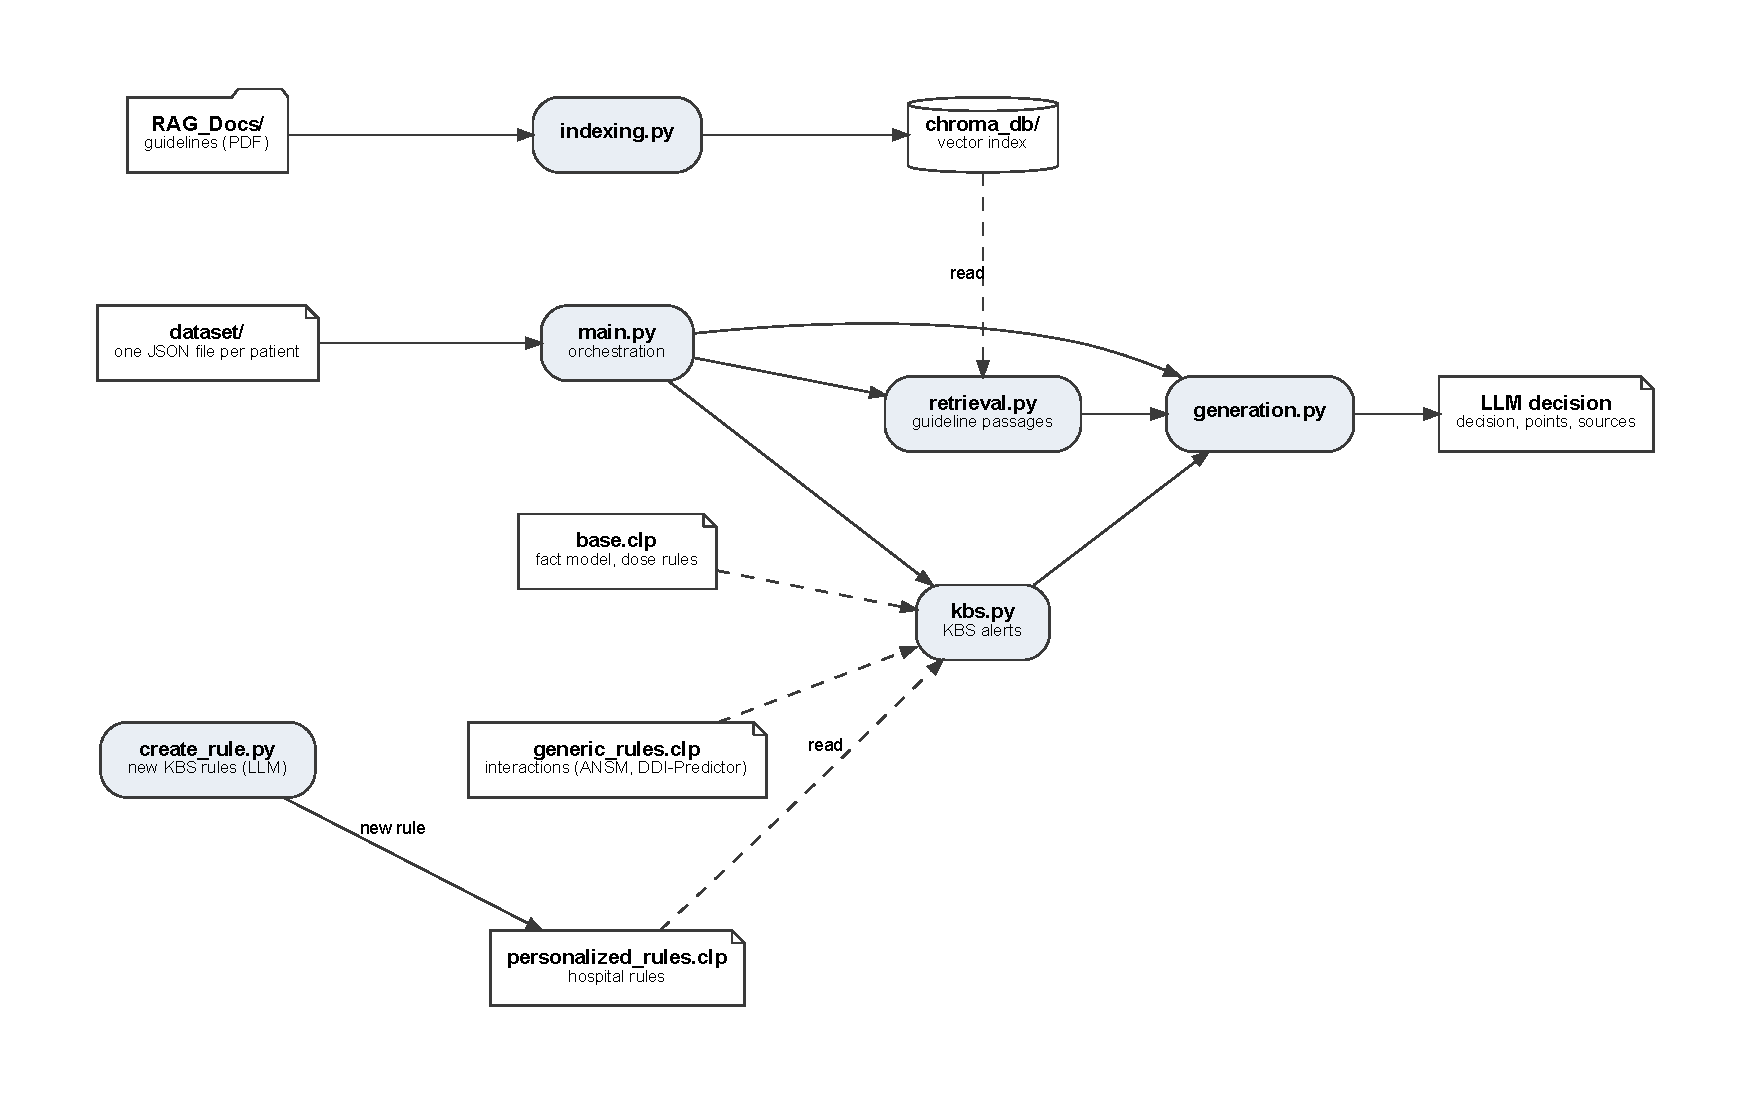
\includegraphics[width=\textwidth]{figures_en/figure_1.pdf}
	\caption{Overall architecture of the pipeline. Guidelines (PDF) are split into passages and indexed in a vector database (ChromaDB). For each patient, the retrieval module extracts relevant passages and the KBS produces deterministic alerts. Both outputs are passed to the language model, which gives the final decision.}
	\label{fig:architecture}
\end{figure}

\subsection{Guideline indexing}

The document base contains clinical guidelines in PDF format. The current version includes the position statement of the French-speaking Diabetes Society (Société Francophone du Diabète, SFD) on the management of type 2 diabetes. % TODO: add the full reference and any other indexed document
Each PDF is converted to text page by page with PyMuPDF4LLM, without optical character recognition. The text of each page is split into passages of 1,500 characters, with an overlap of 200 characters between consecutive passages. Each passage keeps the name of its source file and its page number. Passages are encoded with the Qwen3-Embedding-8B model and stored in a ChromaDB database, using the cosine distance. New documents can be added at any time; they are indexed in the same way.

\subsection{Retrieval of relevant passages}

The retrieval module selects the guideline passages that are useful for a given patient (Figure~\ref{fig:retrieval}). It works in three steps.

\textbf{Detection of abnormal laboratory values.} Each laboratory value is compared with a reference range defined by the pharmacists (for example, 45--110~$\mu$mol/L for serum creatinine and 4--6\% for HbA1c). Values outside the range are converted into short text descriptions, such as ``high serum creatinine''. These descriptions are added to a short clinical profile that also contains the age and weight of the patient.

\textbf{Search for each prescription line.} One query is built for each prescription line. It contains the drug name, dose, unit, dosage regimen and clinical profile. All queries are encoded with the same embedding model as the passages, preceded by a short task instruction, as recommended for this model. For each query, the three closest passages are retrieved from the database.

\textbf{Merging of results.} The same passage can be found by several queries. Duplicates are removed, and the smallest distance is kept for each passage. Passages are then sorted by distance, and the eight closest are kept. Each passage is labelled with its source file and page number, so that the LLM can cite it.

\begin{figure}[ht]
	\centering
	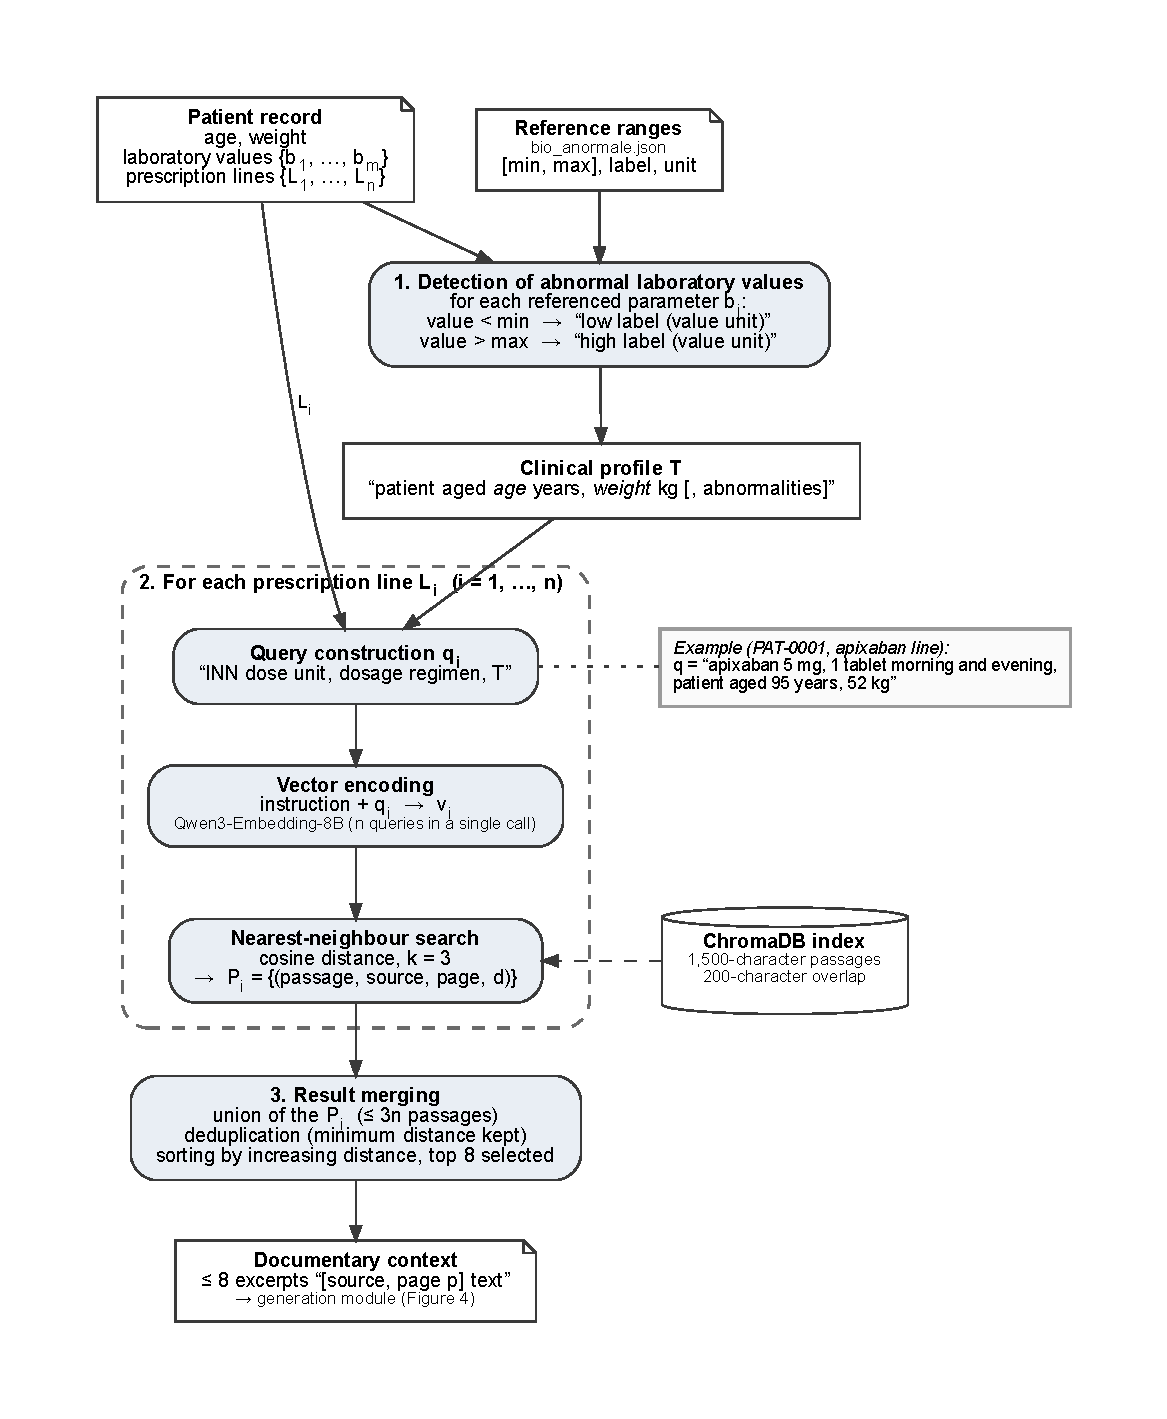
\includegraphics[width=0.75\textwidth]{figures_en/figure_2.pdf}
	\caption{Retrieval of relevant guideline passages for one patient. Abnormal laboratory values are added to the clinical profile. One query is built for each prescription line, encoded with Qwen3-Embedding-8B and used for a 3-nearest-neighbour search (cosine distance). Retrieved passages are deduplicated and sorted by distance; the eight closest form the context passed to the LLM.}
	\label{fig:retrieval}
\end{figure}

\subsection{Knowledge-Based System (KBS)}

The KBS applies deterministic rules to the patient record (Figure~\ref{fig:kbs}). Rules are stored in a JSON file and can be written by pharmacists without programming. Each rule has four fields:
\begin{itemize}
	\item \texttt{medicaments}: drugs that must all be prescribed;
	\item \texttt{conditions}: conditions that must all be true;
	\item \texttt{parmi} and \texttt{minimum}: a list of criteria, of which at least \texttt{minimum} must be true;
	\item \texttt{alerte}: the message returned when the rule is triggered.
\end{itemize}
Only the message is required. A condition compares a variable with a threshold (for example, \texttt{age >= 80}). The variables are the patient characteristics, the laboratory values and the dose of each prescribed drug. A condition on a missing variable is considered false.

The rules are checked one after the other. A rule is triggered when all its fields are satisfied. For example, one rule checks the dose of apixaban: an alert is raised when the dose is not 2.5~mg and the patient meets at least two of the following criteria: age $\geq$ 80 years, weight $\leq$ 60~kg, serum creatinine $\geq$ 133~$\mu$mol/L. The output of the KBS is the list of messages of all triggered rules. This list may be empty.

\begin{figure}[ht]
	\centering
	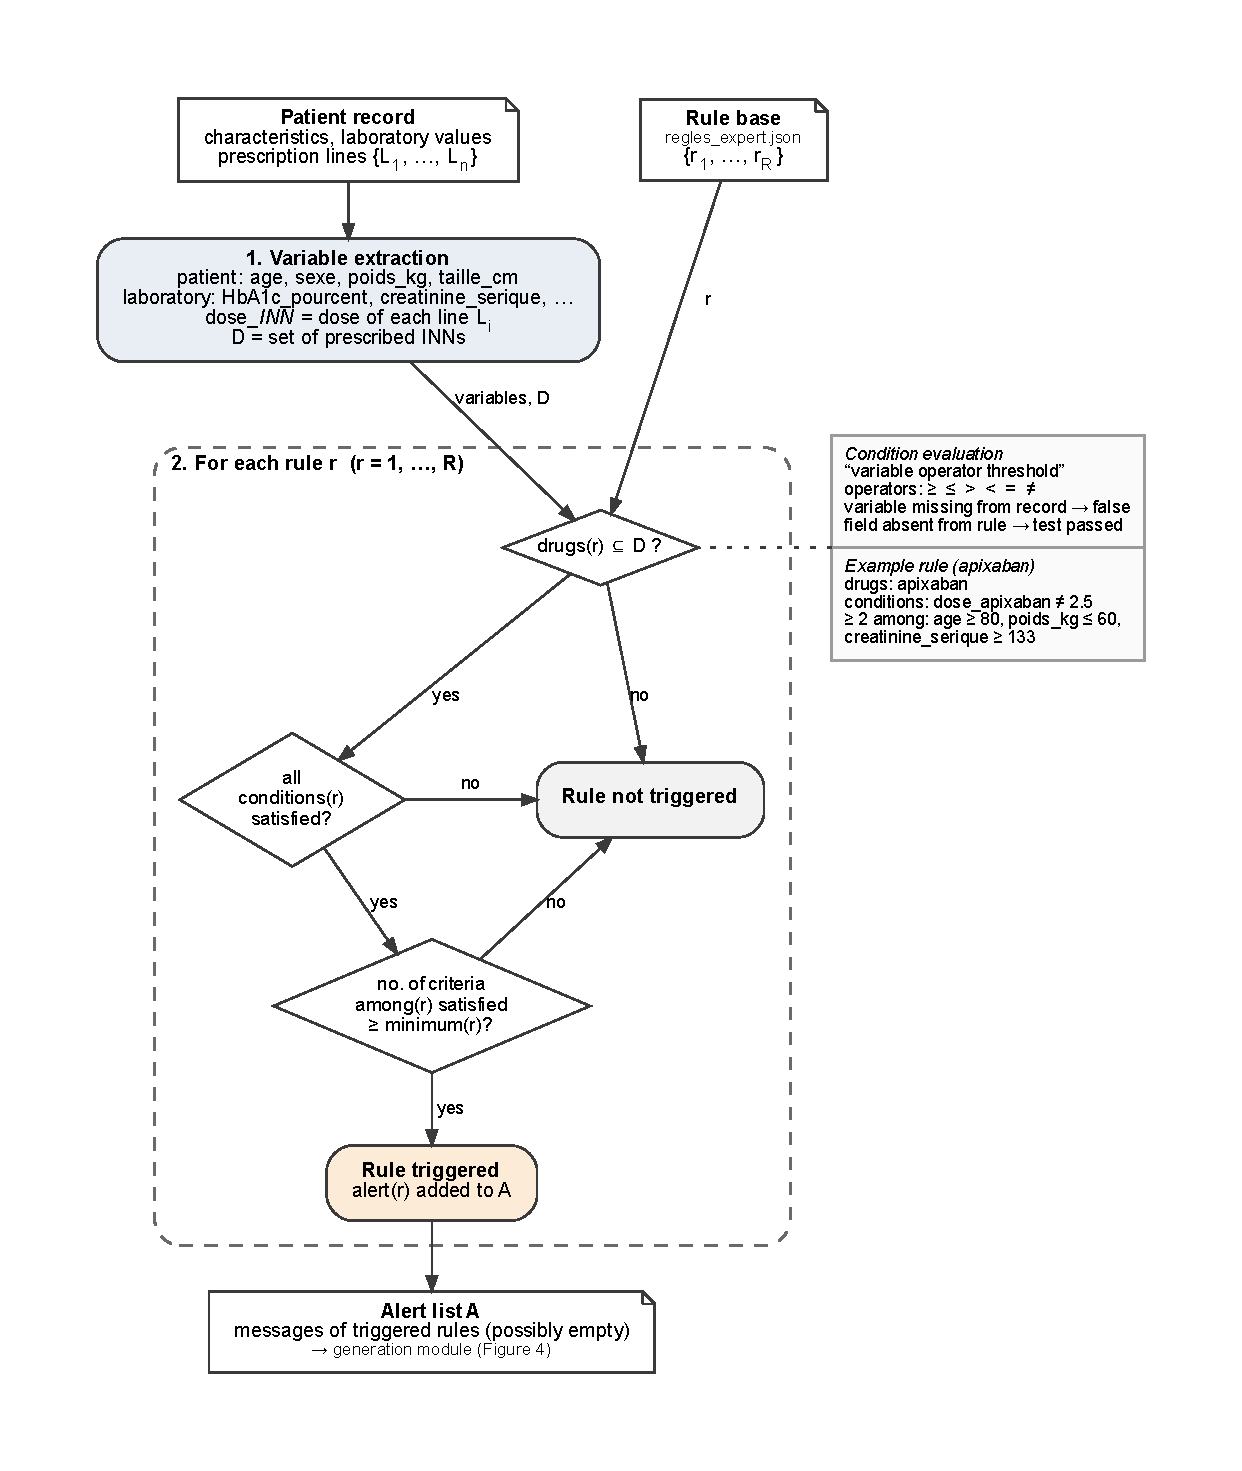
\includegraphics[width=0.75\textwidth]{figures_en/figure_3.pdf}
	\caption{Knowledge-Based System (KBS). Patient variables are extracted from the record. A rule is triggered if (i) all its target drugs are prescribed, (ii) all its mandatory conditions are true and (iii) a minimum number of optional criteria is met. The messages of the triggered rules form the list of alerts passed to the LLM.}
	\label{fig:kbs}
\end{figure}

\subsection{Generation of the pharmaceutical opinion}

The final decision is made by an LLM (Figure~\ref{fig:generation}). We used Qwen3.6-35B-A3B, accessed through the OpenRouter API. The temperature was set to 0 to obtain reproducible answers. The output was limited to 1,024 tokens, the reasoning mode was disabled, and the model was required to answer in JSON format.

The system prompt asks the model to act as a hospital clinical pharmacist. The model must take into account the patient profile (age, weight, laboratory values), the doses, contraindications, drug interactions and French guidelines. It must rely first on the KBS alerts and on the guideline passages when they are provided. The user message contains the patient record in JSON format, followed by the alerts and the retrieved passages.

The model returns three fields:
\begin{itemize}
	\item \texttt{decision}: either ``patient validated'' or ``pharmaceutical intervention proposed'';
	\item \texttt{justification}: three to five sentences. In case of intervention, the justification names the drugs involved, the problem and the proposed change;
	\item \texttt{sources}: the passages used (file and page), and ``KBS'' if an alert was used. The list is empty when the decision relies only on the knowledge of the model.
\end{itemize}

\begin{figure}[ht]
	\centering
	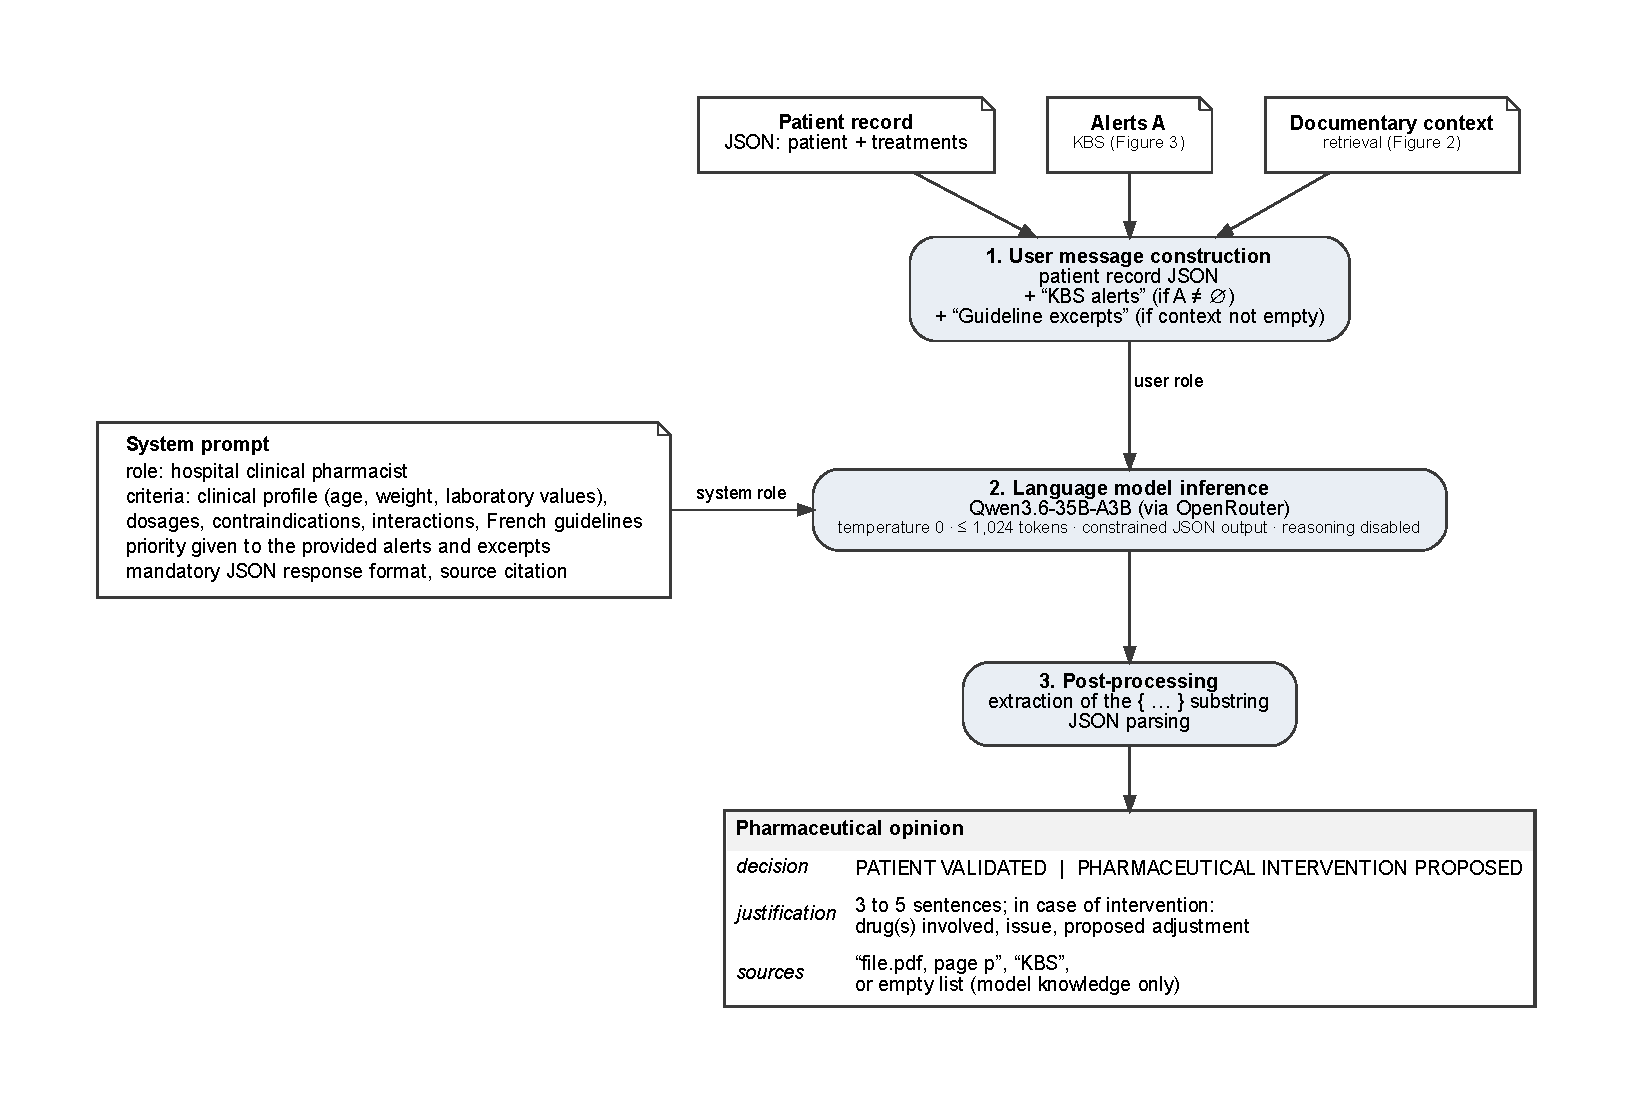
\includegraphics[width=0.85\textwidth]{figures_en/figure_4.pdf}
	\caption{Generation of the pharmaceutical opinion. The user message combines the patient record, the KBS alerts and the retrieved guideline passages. The system prompt defines the role of the model and the analysis criteria. The model (Qwen3.6-35B-A3B, temperature 0, JSON output) returns a decision, a short justification and the cited sources.}
	\label{fig:generation}
\end{figure}

\subsection{Implementation}

The pipeline was written in Python. A graphical interface was built with Streamlit for use by pharmacists. It allows users to run the analysis for all patients or for a single patient, to read the results, and to open the cited sources at the relevant page. It also allows users to add new guidelines to the document base, to add or edit KBS rules, and to update the reference ranges of laboratory values. These changes do not require any programming.

% TODO: Evaluation (dataset, reference standard, metrics)


\section{Results}
\label{sec:results}

% TODO: Performance results

\subsection{Graphical interface}

Figure~\ref{fig:interface_results} shows the main screen of the interface. The top of the screen gives the number of patients, the number of analysed records, and the number of validations and proposed interventions. Records can be filtered by status and searched by patient identifier or drug name. Records that need an action are shown first. For each patient, the interface shows the patient profile, the laboratory values, the prescription, the decision, the justification, the KBS alerts and the cited sources.

Each cited source can be opened with one click. The PDF is then shown at the page cited by the model (Figure~\ref{fig:interface_source}). This allows the pharmacist to check quickly the information used by the model.

\begin{figure}[ht]
	\centering
	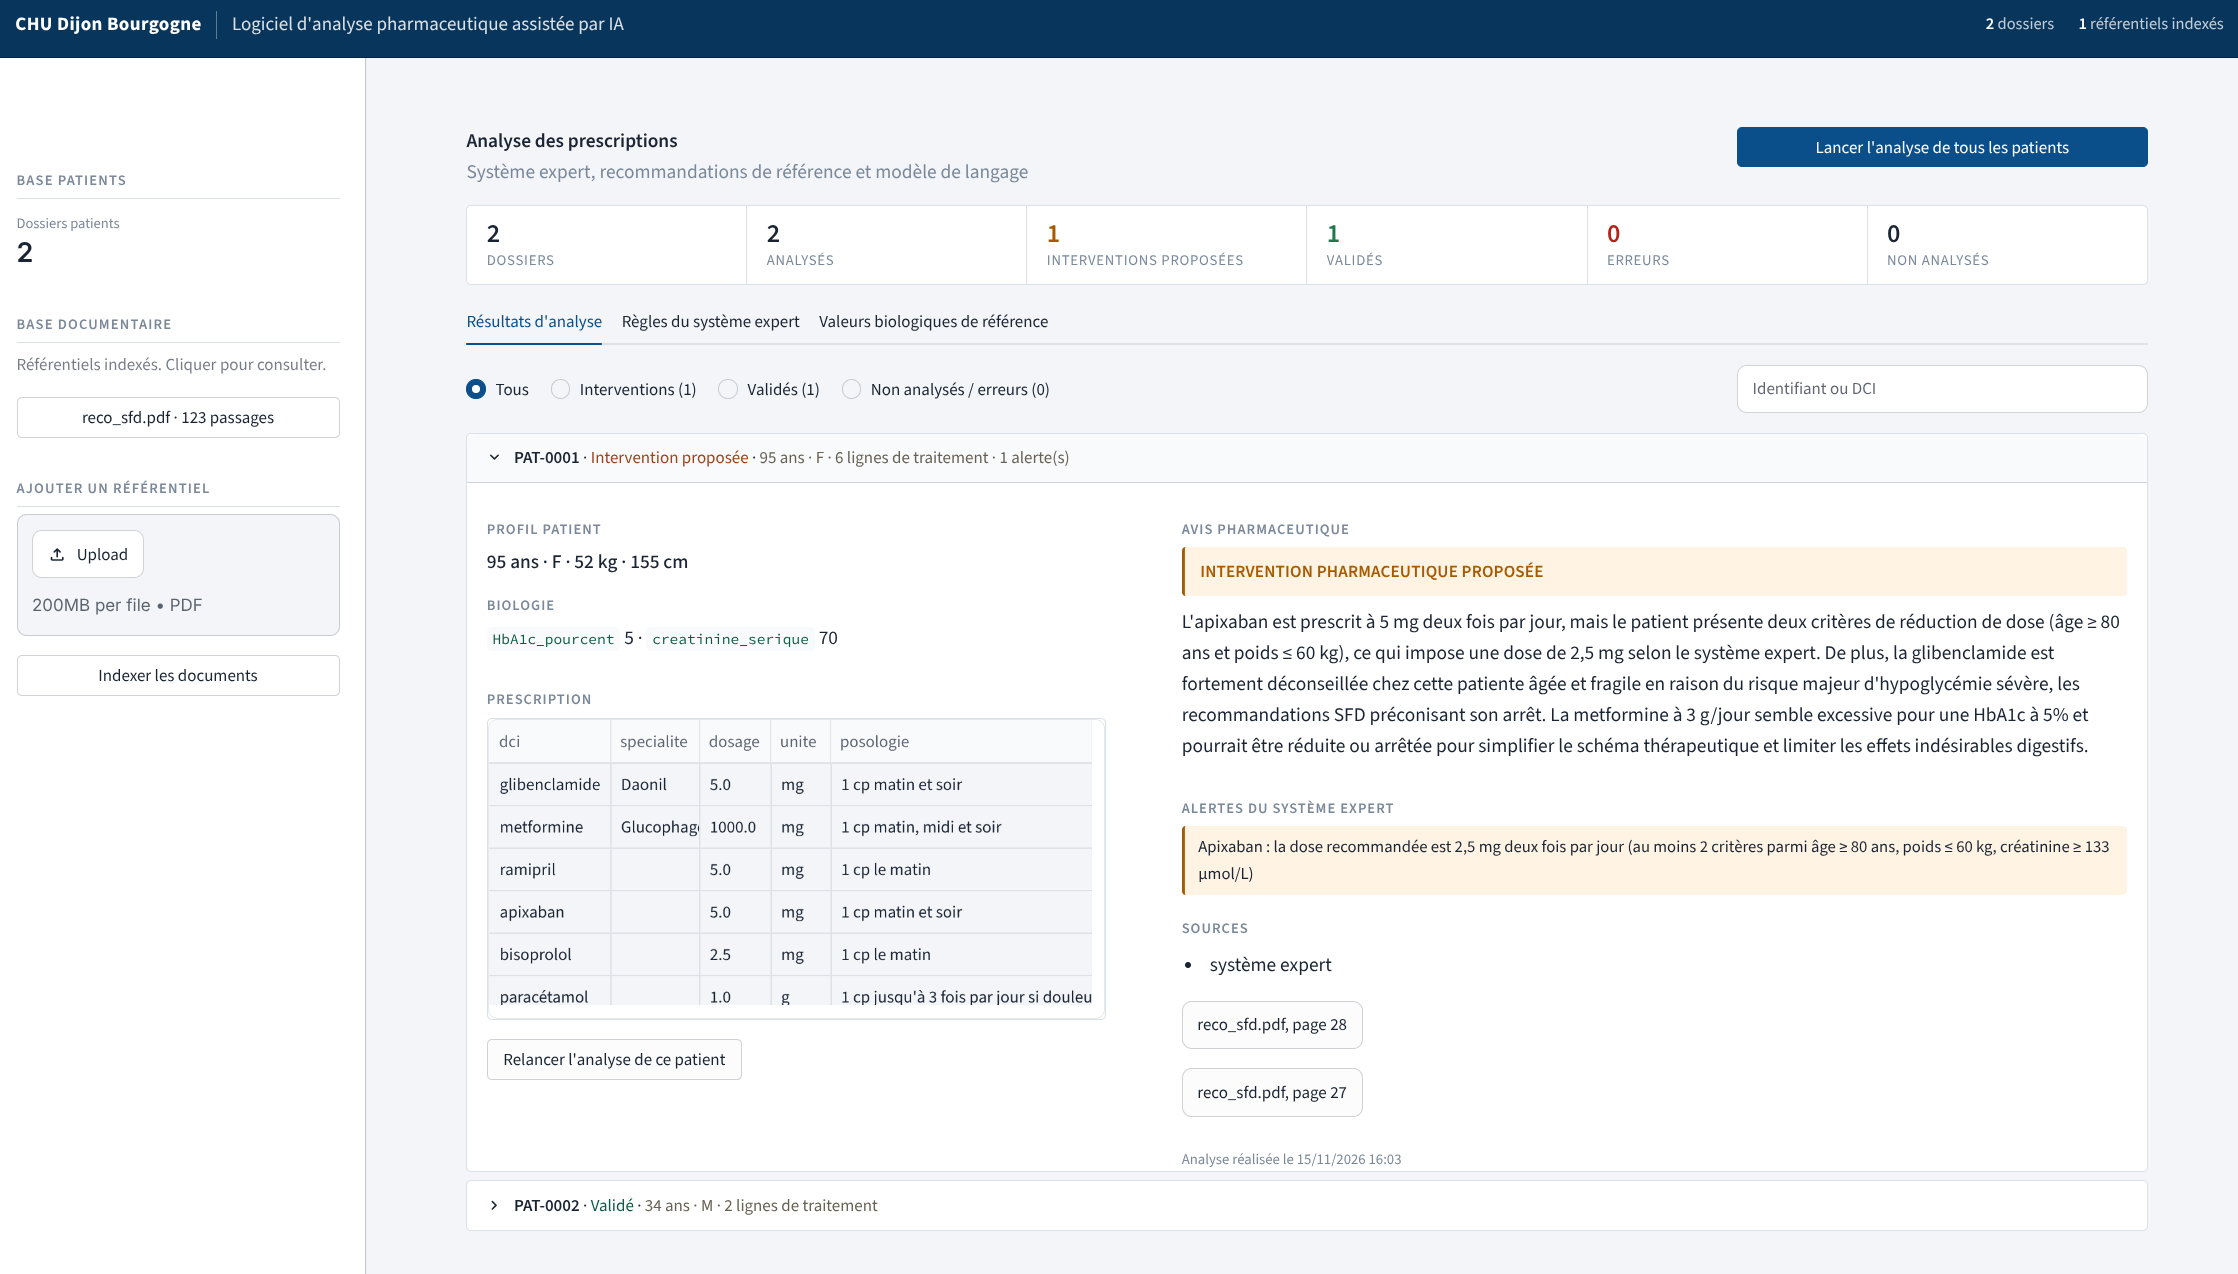
\includegraphics[width=\textwidth]{interface_screenshot_1.png}
	\caption{Main screen of the graphical interface. For each patient, the interface shows the patient profile, the prescription, the pharmaceutical opinion, the KBS alerts and the cited sources.}
	\label{fig:interface_results}
\end{figure}

\begin{figure}[ht]
	\centering
	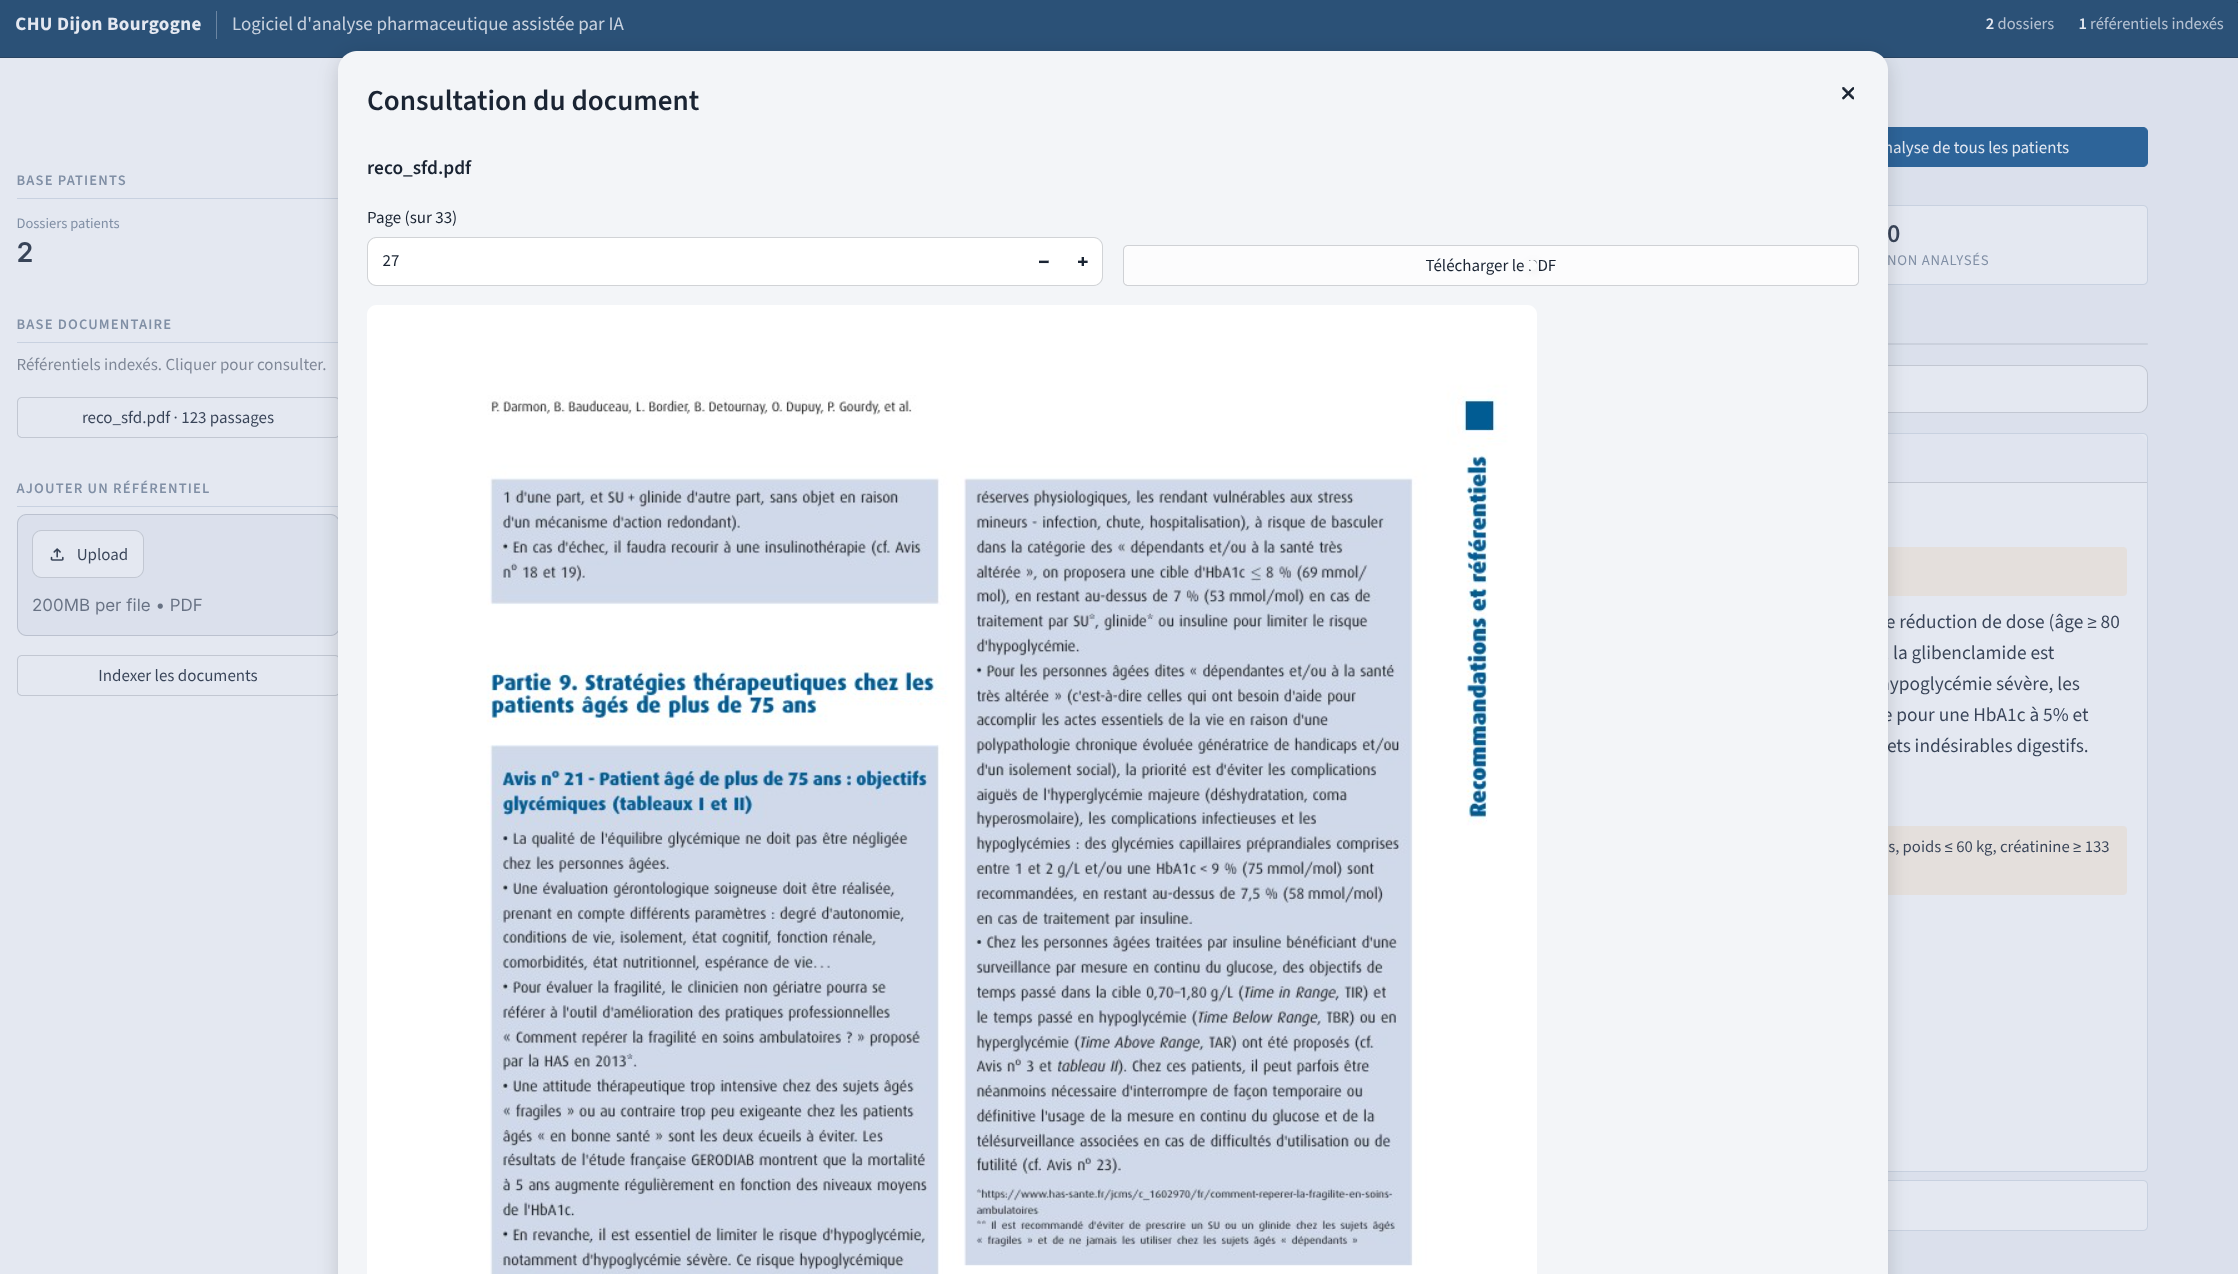
\includegraphics[width=\textwidth]{interface_screenshot_2.png}
	\caption{Display of a cited source. Clicking on a reference opens the guideline document at the page cited by the model.}
	\label{fig:interface_source}
\end{figure}


% TODO: Discussion
% TODO: Conclusion

% \bibliographystyle{unsrtnat}
% \bibliography{references}

\end{document}
